\documentclass[12pt, a4paper]{article}

\usepackage{amssymb}
\usepackage{amsmath}
\usepackage{bm}
\usepackage{geometry}
\usepackage{graphicx}
\usepackage{adjustbox}
\usepackage[font=small,labelfont=bf]{caption}
\usepackage{tikz}
\usetikzlibrary{arrows,automata}
\usepackage[thinlines]{easytable}
\usepackage{hyperref}
\hypersetup{
    colorlinks=true,
    citecolor=black,
    filecolor=black,
    linkcolor=black,
    urlcolor=black
}

\title{Rapport \'Evaluation de performances de r\'eseaux}
\author{Morgane Cadeau, Morgan Canas, Lucas Lafage, William Mateille, Raphael Sombstay}
\date{Novembre 2019}

\makeatletter         
\def\@maketitle{
\raggedright
\begin{center}
\vspace*{\fill}
{\Huge \bfseries \sffamily \@title }\\[4ex] 
{\Large  \@author}\\[4ex] 
\@date\\[8ex]

\includegraphics[width=10cm]{logo-enseeiht}
\vspace*{\fill}
\end{center}}
\makeatother
\renewcommand*\contentsname{Table des mati\`eres}

\begin{document}
\maketitle
\thispagestyle{empty}
\newpage
\tableofcontents

\newpage

\section{Comparaison de files d'attente}
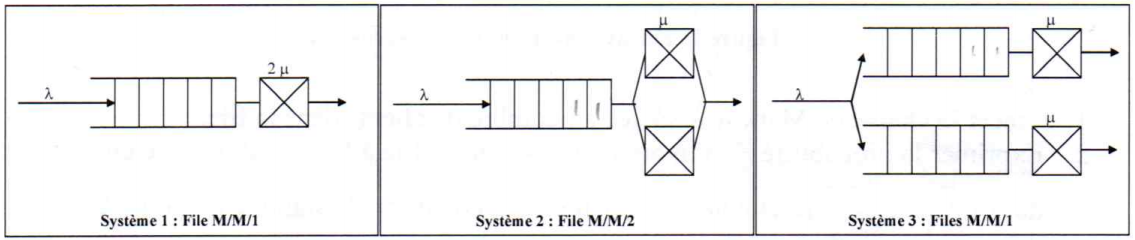
\includegraphics[width=\linewidth]{exercice1}
\captionof{figure}{Sch\'ema des diff\'erents syst\`emes}

\subsection{Temps moyen de r\'eponse du syst\`eme 1}

\quad Calcul du nombre moyen de clients dans la file

\[\rho=\frac{\lambda}{2\mu}\]
\[E[L]=\frac{\rho}{1-\rho} \text{ donc}\]
\[E[L]=\frac{\lambda}{2\mu} * \frac{1}{1-\frac{\lambda}{2\mu}} = \frac{\lambda}{2\mu} * \frac{1}{\frac{2\mu-\lambda}{2\mu}}=\frac{\lambda}{2\mu}*\frac{2\mu}{2\mu-\lambda}\]
\boldmath\[E[L]=\frac{\lambda}{2\mu-\lambda}\]\unboldmath
\linebreak

\quad Calcul du temps moyen de r\'eponse du syst\`eme

\[E[R]=\frac{E[L]}{\lambda}\]
\[E[R]=\frac{\lambda}{2\mu-\lambda}*\frac{1}{\lambda}\]
\boldmath\[E[R]=\frac{1}{2\mu-\lambda}\]\unboldmath
\newpage
\subsection{Temps moyen de r\'eponse du syst\`eme 2}
\medskip

\begin{center}
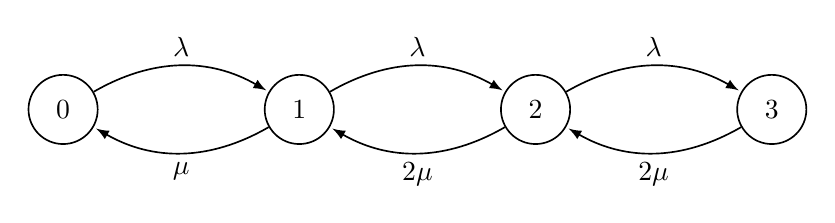
\begin{tikzpicture}[
            > = stealth, % arrow head style
            shorten > = 1pt, % don't touch arrow head to node
            auto,
            node distance = 3cm, % distance between nodes
            semithick % line style
        ]

	\node[state] (0) {$0$};
	\node[state] (1) [right of=0] {$1$};
	\node[state] (2) [right of=1] {$2$};
	\node[state] (3) [right of=2] {$3$};
	
	\draw[-latex,bend left] (0) edge node {$\lambda$} (1);
	\draw[-latex,bend left] (1) edge node {$\mu$} (0);
	\draw[-latex,bend left] (1) edge node {$\lambda$} (2);
	\draw[-latex,bend left] (2) edge node {$2\mu$} (1);
 	\draw[-latex,bend left] (2) edge node {$\lambda$} (3);
	\draw[-latex,bend left] (3) edge node {$2\mu$} (2);
   
\end{tikzpicture}
\captionof{figure}{Cha\^ine de Markov du syst\`eme de 0 \`a 3 clients}
\end{center}
\medskip
On peut donc en d\'eduire la cha\^ine de Markov du syst\`eme pour $n$ clients :
\begin{center}
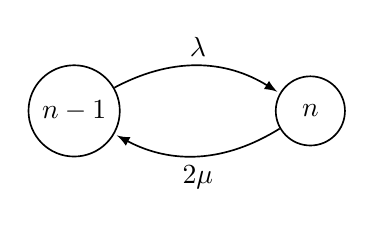
\begin{tikzpicture}[
            > = stealth, % arrow head style
            shorten > = 1pt, % don't touch arrow head to node
            auto,
            node distance = 3cm, % distance between nodes
            semithick % line style
        ]

	\node[state] (A) {$n-1$};
	\node[state] (B) [right of=A] {$n$};
	
 	\draw[-latex,bend left] (A) edge node {$\lambda$} (B);
	\draw[-latex,bend left] (B) edge node {$2\mu$} (A);
   
\end{tikzpicture}
\captionof{figure}{Cha\^ine de Markov du syst\`eme pour $n$ clients}
\end{center}

\bigskip
\quad Utilisation de la m\'ethode des coupes afin de d\'eterminer $\pi_{n}$ selon $\pi_{0}$

\begin{gather*}
\pi_{0}\lambda=\pi_{1}\mu \\
\bm{\pi_{1}=\frac{\lambda}{\mu}\pi_{0}} \\
2\mu\pi_{2}=\lambda\pi_{1}=\frac{\lambda^{2}}{\mu}\pi_{0} \\
\bm{\pi_{2}=\frac{\lambda^{2}}{2\mu^{2}}\pi_{0}} \\
2\mu\pi_{3}=\lambda\pi_{2}=\frac{\lambda^{3}}{2\mu^{2}}\pi_{0} \\
\bm{\pi_{3}=\frac{\lambda^{3}}{4\mu^{3}}\pi_{0}} \\
\text{On a donc }\pi_{n}=\frac{\lambda}{2\mu}\pi_{n-1} \\
\text{On en d\'eduit que }\bm{\pi_{n}=\frac{\lambda^{n}}{2^{n-1}\mu^{n}}\pi_{0}} \\
\text{Or }\rho=\frac{\lambda}{2\mu} \text{ donc } \bm{\pi_{n}=2\rho^{n}\pi_{0}} \\
\end{gather*}

\quad Calcul de $\pi_{0}$ gr\^ace \`a la somme des probabilit\'es

\begin{gather*}
\pi_{0}+\sum_{i=1}^{\infty} \pi_{i} = 1 \\
\pi_{0}=1-\sum_{i=1}^{\infty}\pi_{i} \\
\pi_{0}=1-\sum_{i=1}^{\infty}2\rho^{i}\pi_{0} \\
\pi_{0}=1-2\pi_{0} \sum_{i=1}^{\infty}\rho^{i} \\
\Rightarrow \pi_{0}=1-2\pi_{0}\rho\sum_{i=0}^{\infty}\rho^{i} \\
\pi_{0}=1-2\pi_{0}\rho\left(\frac{1}{1-\rho}\right) \text{ car } \sum_{i=0}^{\infty}\rho^{i}=\frac{1}{1-\rho}\\
\pi_{0}=1-\frac{2\rho}{1-\rho}\pi_{0} \\
\Rightarrow 1 = \pi_{0}+\frac{2\rho}{1-\rho}\pi_{0} \\
1=\pi_{0}\left(1+\frac{2\rho}{1-\rho}\right)=\frac{1-\rho+2\rho}{1-\rho}\pi_{0} \\
\Rightarrow \bm{\pi_{0}=\frac{1-\rho}{1+\rho}} \\
\end{gather*}

\quad La valeur de $\pi_{0}$ nous permet de d\'eduire $\pi_{n}$
\[\bm{\pi_{n}=2\rho^{n}\frac{1-\rho}{1+\rho}}\]

\newpage
\quad Calcul du nombre moyen de clients dans la file

\begin{gather*}
E[L]=\sum_{i=0}^{\infty}i\pi_{i} \\
E[L]=\sum_{i=0}^{\infty}i2\rho^{i}\frac{1-\rho}{1+\rho} \\
E[L]=2\left(\frac{1-\rho}{1+\rho}\right)\sum_{i=0}^{\infty}i\rho^{i} \\
\Rightarrow E[L]=2\left(\frac{1-\rho}{1+\rho}\right)\frac{\rho}{\left(1-\rho\right)^{2}} \text{ car } \sum_{i=0}^{\infty}i\rho^{i} = \frac{\rho}{\left(1-\rho\right)^{2}} \\
E[L]=\frac{2\rho}{\left(1+\rho\right)\left(1-\rho\right)} \\
\Rightarrow \bm{E[L]=\frac{2\rho}{1-\rho^{2}}}
\end{gather*}

\quad Calcul du temps moyen de r\'eponses du syst\`eme 2
\begin{gather*}
E[R]=\frac{E[L]}{\lambda} \\
E[R]=\frac{2\rho}{\lambda\left(1-\rho^{2}\right)} = \frac{2\lambda}{2\mu\lambda\left(1-\rho^{2}\right)} \\
\bm{E[R]=\frac{1}{\mu\left(1-\rho^{2}\right)}}
\end{gather*}

\newpage
\subsection{Nombre moyen de passages d'un client et temps de r\'eponse moyen dans chacune des 2 files du syst\`eme 3}

On peut appliquer le th\'eor\`eme de Jackson car toutes les hypoth\`eses sont respect\'ees
\begin{itemize}
\item Arriv\'ees selon un processus de poisson de d\'ebit $\lambda$
\item Chaque file a 1 seul serveur, un service exponentiel de param\`etre $\mu$, une capacit\'e infinie est est FIFO
\end{itemize}

\medskip
\quad Calcul de la charge $\rho$ 

\begin{gather*}
e_{1} = e_{2} = \frac{1}{2} \\
\lambda_{1} = \lambda_{2} = \frac{1}{2}\lambda \\
\rho_{1} = \rho_{2} = \frac{1}{2}\frac{\lambda}{\mu} = \bm{\frac{\lambda}{2\mu}}
\end{gather*}

\quad Calcul du nombre moyen de passages d'un client dans chacune des 2 files

\begin{gather*}
E[L_{i}] = \frac{\rho_{i}}{1-\rho_{i}} \text{ et on sait que } \rho_{1}=\rho_{2} \\
E[L_{1}] = E[L_{2}] = \frac{\frac{\lambda}{2\mu}}{1-\frac{\lambda}{2\mu}} = \frac{\frac{\lambda}{2\mu}}{\frac{2\mu - \lambda}{2\mu}} \\
E[L_{1}] = E[L_{2}] = \frac{\lambda}{2\mu}\times\frac{2\mu}{2\mu - \lambda} \\
\bm{E[L_{1}] = E[L_{2}] = \frac{\lambda}{2\mu - \lambda}}
\end{gather*}

\quad Calcul du temps moyen de r\'eponse du syst\`eme

\begin{gather*}
E[R_{i}] = \frac{E[L_{i}]}{\lambda e_{i}} \text{ et on sait que } E[L_{1}] = E[L_{2}] \text{ et } e_{1}=e_{2} \\
E[R_{1}]=\frac{E[L_{1}]}{\lambda_{1}}=\frac{\lambda}{2\mu-\lambda}\times\frac{1}{\frac{1}{2}\lambda} \\
E[R_{1}]=\frac{2}{2\mu-\lambda} = \frac{1}{\mu-\frac{1}{2}\lambda}
\end{gather*}

\begin{gather*}
\text{Or } E[L_{1}]=E[L_{2}] \text{ et } \lambda_{1}=\lambda_{2} \text{ donc} \\
\bm{E[R_{1}]=E[R_{2}]=\frac{1}{\mu-\frac{1}{2}\lambda}} \\
E[R]=e_{1}E[R_{1}]+e_{2}E[R_{2} ]\\
E[R]=\frac{1}{2\left(\mu-\frac{1}{2}\lambda\right)}+\frac{1}{2\left(\mu-\frac{1}{2}\lambda\right)} \\
\bm{E[R]=\frac{2}{2\mu-\lambda}=\frac{1}{\mu-\frac{1}{2}\lambda}}
\end{gather*}
\bigskip

\subsection{Classement des 3 syst\`emes en fonction de leurs performances respectives}

\bigskip

\begin{TAB}(r,1cm,1cm)[5pt]{|c|c|c|}{|c|c|c|c|}
	 & Temps moyen de r\'eponse & Temps de r\'eponse pour $\mu=1$ et $\lambda=1$ \\
	 Syst\`eme 1 & $\frac{1}{2\mu-\lambda}$ & 1 \\
	 Syst\`eme 2 & $\frac{1}{\mu\left(1-\rho^{2}\right)}$ & $\frac{4}{3}$ \\
	 Syst\`eme 3 & $\frac{1}{\mu-\frac{1}{2}\lambda}$ & 2 \\
\end{TAB}
\captionof{figure}{Tableau de comparaison des performances des 3 syst\`emes}

\bigskip
\quad Le syst\`eme 1 est le plus efficace car son temps de r\'eponse est plus faible pour la m\^eme valeur de $\mu$ et de $\lambda$ entre les 3 syst\`emes. \medskip

\quad Ce r\'esultat \'etait pr\'evisible car le syst\`eme 1 a un serveur 2 fois plus rapide que les autres syst\`emes. Ainsi, s'il n'y a qu'un client, ce syst\`eme est plus rapide que le syst\`eme 2.

\newpage
\subsection{Performances si on a un syst\`eme 3 bis o\`u les clients se dirigent vers la file la moins remplie}
\quad Dans ce cas l\`a, le syst\`eme 3 bis serait plus performant que le syst\`eme 3 car le temps de r\'eponse serait inf\'erieur. Cependant, le syst\`eme 2 aurait tout de m\^eme un temps moyen de r\'eponse sup\'erieur \`a celui du syst\`eme 2. \medskip

\quad Le classement serait donc le suivant :
\begin{enumerate}
\item Syst\`eme 1
\item Syst\`eme 2
\item Syst\`eme 3 bis
\item Syst\`eme 4
\end{enumerate}

\newpage

\subsection{Montrer que $N(t)=(N1(t),N2(t))$ est markovien et construire la cha\^ine de Markov pour des files inf\'erieures ou \'egales \`a 3}

\begin{center}
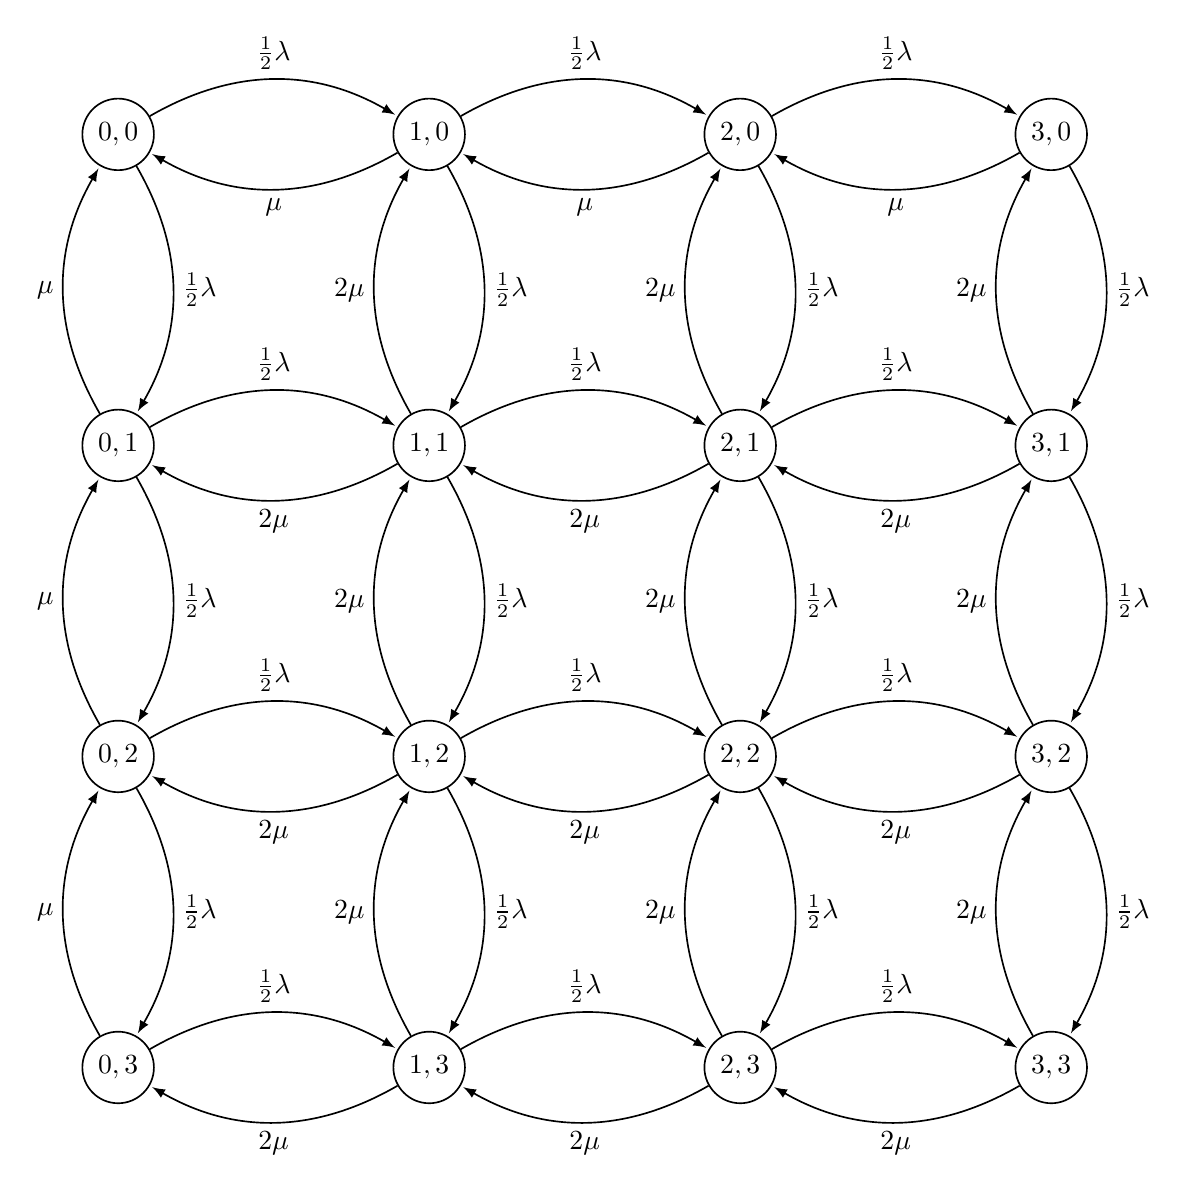
\begin{tikzpicture}[
            > = stealth, % arrow head style
            shorten > = 1pt, % don't touch arrow head to node
            auto,
            node distance = 3.95cm, % distance between nodes
            semithick % line style
        ]

	\node[state] (A) {$0,0$};
	\node[state] (B) [right of=A] {$1,0$};
	\node[state] (C) [right of=B] {$2,0$};
	\node[state] (D) [right of=C] {$3,0$};
	\node[state] (E) [below of=A] {$0,1$};
	\node[state] (F) [right of=E] {$1,1$};
	\node[state] (G) [right of=F] {$2,1$};
	\node[state] (H) [right of=G] {$3,1$};
	\node[state] (I) [below of=E] {$0,2$};
	\node[state] (J) [right of=I] {$1,2$};
	\node[state] (K) [right of=J] {$2,2$};
	\node[state] (L) [right of=K] {$3,2$};
	\node[state] (M) [below of=I] {$0,3$};
	\node[state] (N) [right of=M] {$1,3$};
	\node[state] (O) [right of=N] {$2,3$};
	\node[state] (P) [right of=O] {$3,3$};
	
 	\draw[-latex,bend left] (A) edge node {$\frac{1}{2}\lambda$} (B);
	\draw[-latex,bend left] (B) edge node {$\mu$} (A);
	\draw[-latex,bend left] (B) edge node {$\frac{1}{2}\lambda$} (C);
	\draw[-latex,bend left] (C) edge node {$\mu$} (B);
	\draw[-latex,bend left] (C) edge node {$\frac{1}{2}\lambda$} (D);
	\draw[-latex,bend left] (D) edge node {$\mu$} (C);
	
	\draw[-latex,bend left] (A) edge node {$\frac{1}{2}\lambda$} (E);
	\draw[-latex,bend left] (E) edge node {$\mu$} (A);
	\draw[-latex,bend left] (B) edge node {$\frac{1}{2}\lambda$} (F);
	\draw[-latex,bend left] (F) edge node {$2\mu$} (B);
	\draw[-latex,bend left] (C) edge node {$\frac{1}{2}\lambda$} (G);
	\draw[-latex,bend left] (G) edge node {$2\mu$} (C);
	\draw[-latex,bend left] (D) edge node {$\frac{1}{2}\lambda$} (H);
	\draw[-latex,bend left] (H) edge node {$2\mu$} (D);
	
	\draw[-latex,bend left] (E) edge node {$\frac{1}{2}\lambda$} (F);
	\draw[-latex,bend left] (F) edge node {$2\mu$} (E);
	\draw[-latex,bend left] (F) edge node {$\frac{1}{2}\lambda$} (G);
	\draw[-latex,bend left] (G) edge node {$2\mu$} (F);
	\draw[-latex,bend left] (G) edge node {$\frac{1}{2}\lambda$} (H);
	\draw[-latex,bend left] (H) edge node {$2\mu$} (G);
	
	\draw[-latex,bend left] (E) edge node {$\frac{1}{2}\lambda$} (I);
	\draw[-latex,bend left] (I) edge node {$\mu$} (E);
	\draw[-latex,bend left] (F) edge node {$\frac{1}{2}\lambda$} (J);
	\draw[-latex,bend left] (J) edge node {$2\mu$} (F);
	\draw[-latex,bend left] (G) edge node {$\frac{1}{2}\lambda$} (K);
	\draw[-latex,bend left] (K) edge node {$2\mu$} (G);
	\draw[-latex,bend left] (H) edge node {$\frac{1}{2}\lambda$} (L);
	\draw[-latex,bend left] (L) edge node {$2\mu$} (H);
	
	\draw[-latex,bend left] (I) edge node {$\frac{1}{2}\lambda$} (J);
	\draw[-latex,bend left] (J) edge node {$2\mu$} (I);
	\draw[-latex,bend left] (J) edge node {$\frac{1}{2}\lambda$} (K);
	\draw[-latex,bend left] (K) edge node {$2\mu$} (J);
	\draw[-latex,bend left] (K) edge node {$\frac{1}{2}\lambda$} (L);
	\draw[-latex,bend left] (L) edge node {$2\mu$} (K);
	
	\draw[-latex,bend left] (I) edge node {$\frac{1}{2}\lambda$} (M);
	\draw[-latex,bend left] (M) edge node {$\mu$} (I);
	\draw[-latex,bend left] (J) edge node {$\frac{1}{2}\lambda$} (N);
	\draw[-latex,bend left] (N) edge node {$2\mu$} (J);
	\draw[-latex,bend left] (K) edge node {$\frac{1}{2}\lambda$} (O);
	\draw[-latex,bend left] (O) edge node {$2\mu$} (K);
	\draw[-latex,bend left] (L) edge node {$\frac{1}{2}\lambda$} (P);
	\draw[-latex,bend left] (P) edge node {$2\mu$} (L);
	
	\draw[-latex,bend left] (M) edge node {$\frac{1}{2}\lambda$} (N);
	\draw[-latex,bend left] (N) edge node {$2\mu$} (M);
	\draw[-latex,bend left] (N) edge node {$\frac{1}{2}\lambda$} (O);
	\draw[-latex,bend left] (O) edge node {$2\mu$} (N);
	\draw[-latex,bend left] (O) edge node {$\frac{1}{2}\lambda$} (P);
	\draw[-latex,bend left] (P) edge node {$2\mu$} (O);
\end{tikzpicture}
\captionof{figure}{Cha\^ine de Markov pour des files de longueur inf\'erieures \`a 3}
\end{center}

C'est un processus Markovien car on n'a pas besoin de conna\^itre $N$ pour trouver $N+1$. 
On peut calculer les probabilit\'es suivantes :

\begin{align*}
\text{Probabilit\'e d'une arriv\'ee dans la file : } P(N_{1}(t+dt)=j+1 / N_{1}(t)=j)=\frac{1}{2}\lambda dt + o(dt) \\
\text{Probabilit\'e d'un d\'epart de file : } P(N_{1}(t+dt)=j-1 / N_{1}(t)=j)=\mu dt + o(dt)
\end{align*}

\newpage

\section{File avec arriv\'ees d\'ecourag\'ees}
\begin{center}
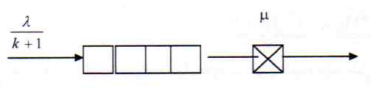
\includegraphics[width=6cm]{exercice2}
\captionof{figure}{Sch\'ema de la file avec arriv\'ees d\'ecourag\'ees}
\end{center}

\subsection{Cha\^ine de Markov associ\'ee au nombre de clients dans la file}
\begin{center}
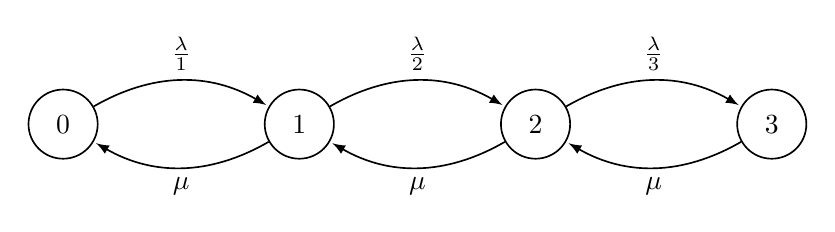
\begin{tikzpicture}[
            > = stealth, % arrow head style
            shorten > = 1pt, % don't touch arrow head to node
            auto,
            node distance = 3cm, % distance between nodes
            semithick % line style
        ]

	\node[state] (0) {$0$};
	\node[state] (1) [right of=0] {$1$};
	\node[state] (2) [right of=1] {$2$};
	\node[state] (3) [right of=2] {$3$};
	
	\draw[-latex,bend left] (0) edge node {$\frac{\lambda}{1}$} (1);
	\draw[-latex,bend left] (1) edge node {$\mu$} (0);
	\draw[-latex,bend left] (1) edge node {$\frac{\lambda}{2}$} (2);
	\draw[-latex,bend left] (2) edge node {$\mu$} (1);
 	\draw[-latex,bend left] (2) edge node {$\frac{\lambda}{3}$} (3);
	\draw[-latex,bend left] (3) edge node {$\mu$} (2);
   
\end{tikzpicture}
\captionof{figure}{Cha\^ine de Markov du syst\`eme de 0 \`a 3 clients}
\end{center}
\medskip
On peut donc en d\'eduire la cha\^ine de Markov du syst\`eme pour $n$ clients :
\begin{center}
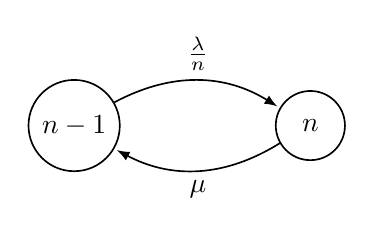
\begin{tikzpicture}[
            > = stealth, % arrow head style
            shorten > = 1pt, % don't touch arrow head to node
            auto,
            node distance = 3cm, % distance between nodes
            semithick % line style
        ]

	\node[state] (A) {$n-1$};
	\node[state] (B) [right of=A] {$n$};
	
 	\draw[-latex,bend left] (A) edge node {$\frac{\lambda}{n}$} (B);
	\draw[-latex,bend left] (B) edge node {$\mu$} (A);
   
\end{tikzpicture}
\captionof{figure}{Cha\^ine de Markov du syst\`eme pour $n$ clients}
\end{center}

\subsection{Probabilit\'e $P_{k}$ d'avoir $k$ clients dans la file. D\'etermination de la condition de stabilit\'e}

\quad Calcul de $\pi_{n}$ par rapport \`a $\pi_{0}$
\begin{gather*}
\pi_{1} = \frac{\lambda}{\mu}\pi_{0} \\
\pi_{2} = \frac{\lambda^{2}}{2\mu^{2}}\pi_{0} \\
\pi_{3} = \frac{\lambda^{3}}{6\mu^{3}}\pi_{0} \\
\bm{\pi_{n} = \frac{\lambda^{n}}{n! \mu^{n}} = \frac{\rho^{n}}{n!} \pi_{0}}
\end{gather*}

\newpage
\quad Calcul de $\pi_{0}$
\begin{gather*}
\pi_{0} = 1 - \sum_{k=1}^{\infty} \pi_{k} \\
\pi_{0} = 1 - \sum_{k=1}^{\infty} \frac{\rho^{k}}{k!} \pi_{0} \\
\pi_{0} = 1 - \pi_{0}\sum_{k=1}^{\infty} \frac{\rho^{k}}{k!} \\
\pi_{0} = 1 - \pi_{0}\left(\sum_{k=0}^{\infty} \frac{\rho^{k}}{k!} - 1 \right) \\
\pi_{0} = 1 - \pi_{0} \left(e^{\rho} - 1 \right) \\
\pi_{0} = 1 - e^{\rho}\pi_{0} + \pi_{0} \\
\bm{\Rightarrow \pi_{0}=\frac{1}{e^{\rho}}}
\end{gather*}

\quad Condition de stabilit\'e de la file \newline 

Le syst\`eme est stable lorsque le d\'ebit d'entr\'ee est inf\'erieur au d\'ebit de sortie. Ici, le d\'ebit d'entr\'ee est variable donc on prend sa valeur maximale lorsque $k=0$. La condition de stabilit\'e est donc \bm{$\lambda<\mu$}.

\bigskip

\subsection{Taux d'utilisation du serveur}

\begin{gather*}
U=1-\pi_{0}=1 - \frac{1}{e^{\rho}} \\
\bm{U=\frac{e^{\rho} - 1}{e^{\rho}}}
\end{gather*}

\newpage
\subsection{Nombre moyen $L$ de clients dans le syst\`eme}

\begin{gather*}
L = \sum_{k=1}^{\infty}k\pi_{k} + 0\times\pi_{0} \\
L = \sum_{k=1}^{\infty}k\frac{\rho^{k}}{k!} \times \frac{1}{e^{\rho}} \\
L = \frac{1}{e^{\rho}} \sum_{k=1}^{\infty}k\frac{\rho^{k}}{k!} \\
L = \frac{\rho}{e^{\rho}} \sum_{k=1}^{\infty} \frac{\rho^{k-1}}{(k-1)!} \\
L = \frac{\rho}{e^{\rho}} \sum_{k-1=0}^{\infty} \frac{\rho^{k-1}}{(k-1)!} \\
L=\frac{\rho}{e^{\rho}}\times e^{\rho} \\
\bm{L=\rho}
\end{gather*}

\subsection{D\'ebit moyen $\Lambda$ en sortie du syst\`eme}

\begin{gather*}
S=\frac{1}{\mu} \\
\Lambda = \frac{U}{S} = U\mu = (1-\pi_{0})\mu \\
\bm{\Lambda = \frac{\mu(e^{\rho} - 1)}{e^{\rho}}}
\end{gather*}

\subsection{D\'emonstration que le temps moyen de r\'eponse de cette file est $R=\frac{\rho}{\mu(1-\pi_{0})}$}

\begin{gather*}
L=R\Lambda \\
\Rightarrow R = \frac{L}{\Lambda} = \frac{\rho}{U\mu} \\
\text{Donc on retrouve } \bm{R = \frac{\rho}{(1-\pi_{0})\mu}}
\end{gather*}

\newpage

\section{Unit\'e de transmission de paquets}
\subsection{Notation de Kendall de la file}

La file pr\'esent\'ee a une arriv\'ee de paquets qui suit une loi exponentielle, ceux-ci ont une longueur exponentiellement ditribu\'ee. Ainsi, leur temps de service suit une loi exponentielle. Enfin, il n'y a qu'un commutateur. La notation de Kendall de la file se note donc \bm{$M/M/1$}.

\subsection{Nombre moyen de paquets dans la file et temps moyen de r\'eponse}

\begin{gather*}
\rho=\frac{\lambda}{\mu C} \\
\mu C=\frac{10000000}{1000}=10000 \\
L=\frac{\lambda}{\mu C-\lambda} \\
R = \frac{1}{\mu C - \lambda}
\end{gather*}

\subsubsection{Charge de trafic \`a $0.6$}

\begin{gather*}
\rho = 0.6 = \frac{\lambda}{10000} \Rightarrow \lambda = 6000 \\
L = \frac{\lambda}{\mu C - \lambda} = \frac{6000}{10000 - 6000} \\
\bm{L = \frac{3}{2}} \\
R = \frac{1}{\mu C - \lambda} = \frac{1}{10000 - 6000} = \frac{1}{4000} \\
\bm{R = 0,25.10^{-3}} \\
\end{gather*}

\subsubsection{Charge de trafic \`a $0.9$}

\begin{gather*}
\rho = 0.9 = \frac{\lambda}{10000} \Rightarrow \lambda = 9000 \\
L = \frac{\lambda}{\mu C - \lambda} = \frac{9000}{10000 - 9000} \\
\bm{L = 9} \\
R = \frac{1}{\mu C - \lambda} = \frac{1}{10000 - 9000} = \frac{1}{1000} \\
\bm{R = 0,1.10^{-2}} \\
\end{gather*}

\subsection{Cas de paquets de longueur constante}

\subsubsection{Charge de trafic \`a $0.6$}

\begin{gather*}
E[L] = \frac{\rho(2-\rho)}{2(1-\rho)} = \frac{0,6(2-0,6)}{2(1-0,6)} \\
\bm{E[L] = 1,05} \\
E[R] = \frac{\rho(2-\rho)}{2\lambda(1-\rho)} = \frac{0,6(2-0,6)}{2\times6000(1-0,6)} \\
\bm{E[R] =0,175ms}
\end{gather*}

\subsubsection{Charge de trafic \`a $0.9$}

\begin{gather*}
E[L] = \frac{\rho(2-\rho)}{2(1-\rho)} = \frac{0,9(2-0,9)}{2(1-0,9)} \\
\bm{E[L] = 4,95} \\
E[R] = \frac{\rho(2-\rho)}{2\lambda(1-\rho)} = \frac{0,9(2-0,9)}{2\times6000(1-0,9)} \\
\bm{E[R] =0,55ms}
\end{gather*}

\newpage

\section{R\'eseaux de commutateurs}
\subsection{Temps moyen de r\'eponse}
\subsubsection{Paquets de longueur exponentiellement distribu\'ee}
\quad Calcul du temps moyen de r\'eponse de chacune des files

\medskip
\textbf{Switch 1 et 2}

\begin{gather*}
E[R] = \frac{1}{\mu - \lambda} \text{ car les files sont de la forme } M/M/1 \\
\rho = 0.5 \text{ donc } \mu = 2\lambda \\
E[R_{1}]=E[R_{2}]=\frac{1}{\mu-\lambda} \\
\bm{E[R_{1}]=E[R_{2}]=\frac{1}{\lambda}} 
\end{gather*}

\textbf{Switch 3}

\begin{gather*}
\lambda_{31} = 0,5\lambda + 0,5\lambda = \lambda \text{ donc } e_{31}=1 \\
\lambda_{32} = 0,5\lambda + 0,5\lambda = \lambda \text{ donc } e_{32}=1 \\
\rho_{31}=\frac{\lambda_{31}}{\mu_{31}} = \frac{\lambda}{\mu} = \frac{\lambda}{2\lambda}=\frac{1}{2} \\
\rho_{32}=\frac{\lambda_{32}}{\mu_{32}} = \frac{\lambda}{\mu} = \frac{\lambda}{2\lambda}=\frac{1}{2} \\
E[L_{i}] = \frac{\rho_{i}}{1-\rho_{i}} = \frac{0,5}{1-0,5} = 1 \\
E[R_{i}] = \frac{E[L_{i}]}{\lambda} = \frac{1}{\lambda} \\\\
\text{On trouve donc les r\'esultats suivants} \\
\bm{E[L_{31}] = 1} \\
\bm{E[R_{31}] = \frac{1}{\lambda}} \\
\bm{E[L_{32}] = 1} \\
\bm{E[R_{32}] = \frac{1}{\lambda}} \\
\end{gather*}

\quad Temps moyen de r\'eponse de l'ensemble

\medskip

\begin{gather*}
E[R_{3}]=0,5E[R_{31}]+0,5E[R_{32}] = \frac{1}{\lambda} \\
E[R] = 0,5E[R_{1}] + 0,5E[R_{2}] + E[R_{3}] \\
\bm{E[R] = \frac{2}{\lambda}} \\
\end{gather*}

\subsubsection{Paquets de taille constante}

\quad Calcul du temps moyen de r\'eponse de chacune des files

\medskip
\textbf{Switch 1 et 2}

\begin{gather*}
E[R]=\frac{\rho(2-\rho)}{2\lambda(1-\rho)} = \frac{0,5(2-0,5)}{2\lambda(1-0,5)} \\
\bm{E[R] = \frac{3}{4\lambda}}
\end{gather*}

\textbf{Switch 3}

\begin{gather*}
\bm{E[R_{31}] = \frac{3}{4\lambda}} \\
\bm{E[R_{32}] = \frac{3}{4\lambda}} \\
\end{gather*}

\quad Temps moyen de r\'eponse de l'ensemble

\medskip

\begin{gather*}
E[R_{3}]=0,5E[R_{31}]+0,5E[R_{32}] = \frac{3}{4\lambda} \\
E[R] = 0,5E[R_{1}] + 0,5E[R_{2}] + E[R_{3}] \\
\bm{E[R] = \frac{3}{2\lambda}} \\
\end{gather*}

\subsection{Temps moyen de r\'eponse du sch\'ema simplifi\'e}
\subsubsection{Paquets de longueur exponentiellement distribu\'ee}

\begin{gather*}
E[R]=\frac{1}{\mu -\lambda} \text{ et } \mu=2\lambda \\
\bm{E[R_{1}] = \frac{1}{2\lambda - \lambda} = \frac{1}{\lambda}} \\
\\ \text{On a } \rho < 1 \text{ donc } \Lambda = \lambda \\
\bm{E[R_{1}] = \frac{1}{2\lambda - \lambda} = \frac{1}{\lambda}} \\
E[R] = E[R_{1}] + E[R_{2}] \\
\bm{E[R] = \frac{2}{\lambda}}
\end{gather*}

\subsubsection{Paquets de taille constante}

\begin{gather*}
E[R] = \frac{\rho(2-\rho}{2\lambda(1-\rho)} \\
E[R_{1}]=\frac{0,5(2-0,5)}{2\lambda(1-0,5)} \\
\bm{E[R_{1}]=\frac{3}{4\lambda}}\\
E[R_{2}]=\frac{0,5(2-0,5)}{2\lambda(1-0,5)} \\
\bm{E[R_{2}]=\frac{3}{4\lambda}}\\
\bm{E[R] = E[R_{1}] + E[R_{2}] = \frac{3}{2\lambda}}
\end{gather*}
\bigskip

On constate que le sch\'ema simplifi\'e est \'equivalent au sch\'ema complet pour $E[R]$. En ce qui concerne la diff\'erence entre les paquets de taille constante et de longueur exponentiellement distribu\'ee, on peut voir que le temps de r\'eponse est l\'eg\`erement sup\'erieur pour des paquets de longueur exponentiellement distribu\'ee.

\newpage
\subsection{Mod\'elisation du nouveau syst\`eme et temps moyen de r\'eponse}

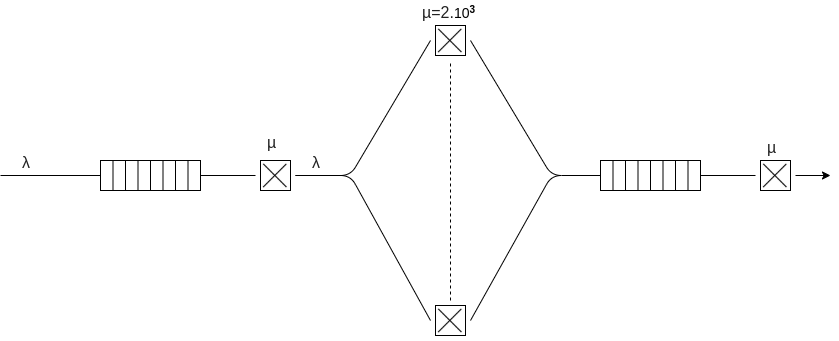
\includegraphics[width=\linewidth]{exercice4}
\captionof{figure}{Mod\'elisation du nouveau syst\`eme}

\begin{gather*}
\text{Pour une file } M/M/N \text{, on sait que  } E[R]=\frac{1}{\mu} \\
\text{Or, on sait que } E[R_{File M/M/N}] = 0,5.10^{-3} \\
\text{Donc, on a } 0,5.10^{-3} = \frac{1}{\mu} \iff \mu = 2.10^{3} \\
\text{On a alors } E[R_{N}] = E[R] + E[R_{File M/M/N}] \\
\bm{E[R_{N}] = \frac{2}{\lambda} + 0,5.10^{-3} s}
\end{gather*}

\newpage
\section{\'Economie d'\'energie d'un serveur vid\'eo}
\subsection{V\'erification que $\{Dt, t \ge 0\}$ constitue une cha\^ine de Markov}

\begin{gather*}
P(Dt(t+dt)=j+1 / Dt(t)=j)=\lambda dt + o(dt) \\
P(Dt(t+dt)=j-1 / Dt(t)=j)=\mu dt + o(dt) \\
\end{gather*}

On a donc un processus Markovien car le passage d'un \'etat \`a un autre ne d\'epend pas des \'etats pr\'ec\'edents.
\bigskip

\begin{center}
...
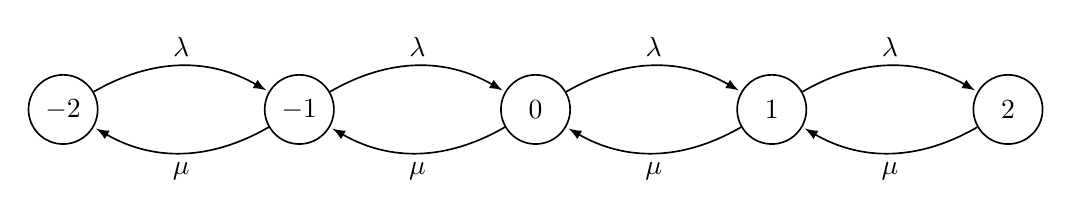
\begin{tikzpicture}[
            > = stealth, % arrow head style
            shorten > = 1pt, % don't touch arrow head to node
            auto,
            node distance = 3cm, % distance between nodes
            semithick % line style
        ]

	\node[state] (-2) {$-2$};
	\node[state] (-1) [right of=-2] {$-1$};
	\node[state] (0) [right of=-1] {$0$};
	\node[state] (1) [right of=0] {$1$};
	\node[state] (2) [right of=1] {$2$};
	
	\draw[-latex,bend left] (-2) edge node {$\lambda$} (-1);
	\draw[-latex,bend left] (-1) edge node {$\mu$} (-2);
	\draw[-latex,bend left] (-1) edge node {$\lambda$} (0);
	\draw[-latex,bend left] (0) edge node {$\mu$} (-1);
	\draw[-latex,bend left] (0) edge node {$\lambda$} (1);
	\draw[-latex,bend left] (1) edge node {$\mu$} (0);
	\draw[-latex,bend left] (1) edge node {$\lambda$} (2);
	\draw[-latex,bend left] (2) edge node {$\mu$} (1);
   
\end{tikzpicture}
...
\end{center}
\captionof{figure}{Cha\^ine de Markov du syst\`eme}

\subsection{La cha\^ine n'est jamais ergodique}
La cha\^ine n'est jamais ergodique car elle a un nombre infini d'\'etat.
\begin{gather*}
\text{Si } \lambda > \mu \text{, } Dt \text{ va tendre vers } +\infty \\
\text{Si } \mu > \lambda \text{, } Dt \text{ va tendre vers } -\infty \\
\text{Si } \lambda = \mu \text{, } Dt \text{ va tendre vers } 0 \\
\end{gather*}
On ne pourra donc pas explorer toute la cha\^ine.

\subsection{Valeurs de $Dt$ avec une capacit\'e limit\'ee C}

\begin{gather*}
0<Rt<C \text{ et } 0<Vt<C \\
\end{gather*}
Donc la diff\'erence $Dt$ est comprise entre $-C$ et $C$.
\bigskip
\begin{gather*}
\bm{Dt \in [-C; C]}
\end{gather*}

\newpage
\subsection{V\'erification que $\{Dt, t \ge 0\}$ constitue une cha\^ine de Markov avec une capacit\'e limit\'ee C}
On ne change rien aux param\`etres de d\'epart. Les paquets arrivent toujours de mani\`ere poissonienne, on a donc un processus Markovien.

\begin{center}
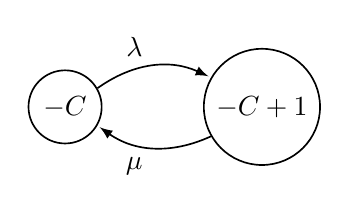
\begin{tikzpicture}[
            > = stealth, % arrow head style
            shorten > = 1pt, % don't touch arrow head to node
            auto,
            node distance = 2.5cm, % distance between nodes
            semithick % line style
        ]

	\node[state] (C) {$-C$};
	\node[state] (C2) [right of=C] {$-C+1$};
	
	\draw[-latex,bend left] (C) edge node {$\lambda$} (C2);
	\draw[-latex,bend left] (C2) edge node {$\mu$} (C);
   
\end{tikzpicture}
...
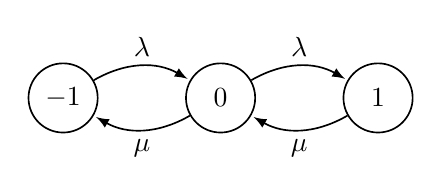
\begin{tikzpicture}[
            > = stealth, % arrow head style
            shorten > = 1pt, % don't touch arrow head to node
            auto,
            node distance = 2cm, % distance between nodes
            semithick % line style
        ]

	\node[state] (-1) {$-1$};
	\node[state] (0) [right of=-1] {$0$};
	\node[state] (1) [right of=0] {$1$};
	
	\draw[-latex,bend left] (-1) edge node {$\lambda$} (0);
	\draw[-latex,bend left] (0) edge node {$\mu$} (-1);
	\draw[-latex,bend left] (0) edge node {$\lambda$} (1);
	\draw[-latex,bend left] (1) edge node {$\mu$} (0);
   
\end{tikzpicture}
...
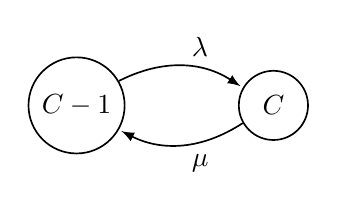
\begin{tikzpicture}[
            > = stealth, % arrow head style
            shorten > = 1pt, % don't touch arrow head to node
            auto,
            node distance = 2.5cm, % distance between nodes
            semithick % line style
        ]

	\node[state] (C) {$C-1$};
	\node[state] (C2) [right of=C] {$C$};
	
	\draw[-latex,bend left] (C) edge node {$\lambda$} (C2);
	\draw[-latex,bend left] (C2) edge node {$\mu$} (C);
   
\end{tikzpicture}
\end{center}
\captionof{figure}{Cha\^ine de Markov du syst\`eme \`a temps continu}

\subsection{Probabilit\'es stationnaires des \'etats en fonction de $\rho$ et $C$}

\begin{gather*}
\rho = \frac{\lambda}{\mu} \\
\pi_{0}\lambda=\mu\pi_{1} \Rightarrow\pi_{1}=\frac{\lambda}{\mu}\pi_{0} \\
\pi_{1} = \rho\pi_{0} \\
\pi_{0}\mu = \pi_{-1}\lambda \Rightarrow \pi_{-1} = \frac{\mu}{\lambda}\pi_{0} \\
\pi_{-1} = \rho^{-1}\pi_{0} \\
\pi_{2} = \rho\pi_{1} \Rightarrow \pi_{2}=\rho^{2}\pi_{0} \\
\pi_{-2} = \rho^{-1}\pi_{-1} \Rightarrow \pi_{-2}=\rho^{-2}\pi_{0} \\
\text{On a donc } \bm{\pi_{k}=\rho^{k}\pi_{0}} \text{ pour } \rho\neq1
\end{gather*}

\begin{gather*}
\text{Pour une file } M/M/1/N \text{, on sait que } \pi_{0}=\frac{1-\rho}{1-\rho^{C+1}} \\
\text{On a donc } \bm{\pi_{k}=\rho^{k} \times \frac{1-\rho}{1-\rho^{C+1}}} \\
\text{Et si } \rho = 1 \text{, on a } \pi_{k} = \frac{1}{C+1}
\end{gather*}

\newpage
\section{Syst\`eme cyclique-multiserveur}
\subsection{\'Etablissement de la cha\^ine de Markov des taux de transition}
On d\'efinit nos \'etats de cette fa\c{c}on : (nb client file 1, nb client file 2)
\begin{center}
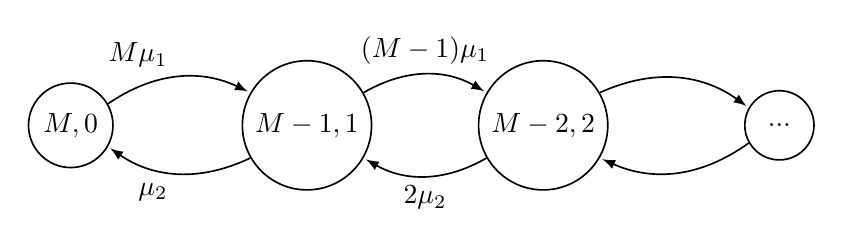
\begin{tikzpicture}[
            > = stealth, % arrow head style
            shorten > = 1pt, % don't touch arrow head to node
            auto,
            node distance = 3cm, % distance between nodes
            semithick % line style
        ]

	\node[state] (1) {$M, 0$};
	\node[state] (2) [right of=1] {$M-1, 1$};
	\node[state] (3) [right of=2] {$M-2, 2$};
	\node[state] (p) [right of=3] {$...$};
	
	\draw[-latex,bend left] (1) edge node {$M\mu_{1}$} (2);
	\draw[-latex,bend left] (2) edge node {$\mu_{2}$} (1);
	\draw[-latex,bend left] (2) edge node {$(M-1)\mu_{1}$} (3);
	\draw[-latex,bend left] (3) edge node {$2\mu_{2}$} (2);
	\draw[-latex,bend left] (3) edge node {} (p);
	\draw[-latex,bend left] (p) edge node {} (3);
	
   
\end{tikzpicture}

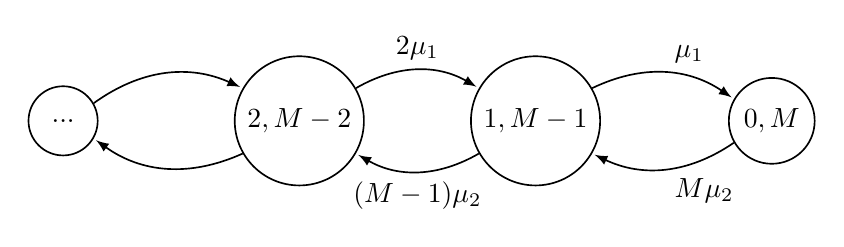
\begin{tikzpicture}[
            > = stealth, % arrow head style
            shorten > = 1pt, % don't touch arrow head to node
            auto,
            node distance = 3cm, % distance between nodes
            semithick % line style
        ]
        
    \node[state] (p) {$...$};
	\node[state] (4) [right of=p] {$2, M-2$};
	\node[state] (5) [right of=4] {$1, M-1$};
	\node[state] (6) [right of=5] {$0, M$};
	
	\draw[-latex,bend left] (p) edge node {} (4);
	\draw[-latex,bend left] (4) edge node {} (p);
	\draw[-latex,bend left] (4) edge node {$2\mu_{1}$} (5);
	\draw[-latex,bend left] (5) edge node {$(M-1)\mu_{2}$} (4);
	\draw[-latex,bend left] (5) edge node {$\mu_{1}$} (6);
	\draw[-latex,bend left] (6) edge node {$M\mu_{2}$} (5);
   
\end{tikzpicture}
\captionof{figure}{Cha\^ine de Markov du syst\`eme}
\end{center}
\bigskip

\subsection{V\'erifions si la propriété PASTA s'applique dans ce syst\`eme}
Pour que la propri\'et\'e PASTA s'applique, il faut que la propabilit\'e d'\'etat vue d'un client se pr\'esentant dans le syst\`eme doit être \'egale \`a la propabilit\'e d'\'etat stationnaire.

\medskip
Elle ne s'applique pas dans ce syst\`eme car la probabilit\'e d'\'etat vue d'un client n'est pas \'egale \`a la probabilit\'e d'\'etat stationnaire car la probabilit\'e d'arriv\'ee varie selon l'\'etat courant.

\subsection{D\'etermination des Pk et de la condition d'ergodicit\'e du syst\`eme}
On utilise la technique des coupes :
\begin{gather*}
\bm{\pi_{(1,M-1)} = \frac{M\mu_{2}}{\mu_{1}}\pi_{(0,M)}} \\\\
\pi_{(2,M-2)} = \frac{(M-1)\mu_{2}}{2\mu_{1}}\pi_{(1,M-1)} \\
\bm{\pi_{(2,M-2)} = \frac{(M-1)M\mu_{2}^{2}}{2\mu_{1}^{2}}\pi_{(0,M)}} \\\\
\pi_{(3,M-3)} = \frac{(M-2)\mu_{2}}{3\mu_{1}}\pi_{(2,M-2)} \\
\bm{\pi_{(3,M-3)} = \frac{(M-2)(M-1)M\mu_{2}^{3}}{6\mu_{1}^{3}}\pi_{(0,M)}}
\end{gather*}

On en déduit donc :
\begin{gather*}
\pi_{(k,M-k)} = \frac{\mu_{2}^{k}\times \frac{M!}{(M-k)!}}{k!\mu_{1}^{k}}\pi_{(0,M)} \\
\bm{\pi_{(k,M-k)} = \left(\frac{\mu_{2}}{\mu_{1}}\right)^{k}\times \frac{M!}{k!(M-k)!}\pi_{(0,M)}}
\end{gather*}

Pour que la cha\^ine soit ergodique, il faut que la cha\^ine de markov ait un nombre fini d'\'etats, qu'elle soit irr\'eductible et ap\'eriodique. Dans notre cas, il faut donc que M soit fini pour avoir un nombre d'\'etats fini.

\subsection{Temps de r\'eponse moyen}

\begin{gather*}
E[R_{1}]=\frac{1}{\mu_{1}} \\
E[R_{2}] = \frac{1}{\mu_{2}} \\
\text{Donc } \bm{E[R] = \frac{1}{\mu_{1}} + \frac{1}{\mu_{2}}}
\end{gather*}

\end{document}
